\documentclass[tikz]{standalone}

\usepackage{amsmath}
\usepackage{unicode-math}
\usepackage{mathtools}
\usepackage{derivative}

\setmainfont{Stix Two Text}
\setmathfont{Stix Two Math}

\usetikzlibrary{arrows.meta,fit,positioning}

\renewcommand{\familydefault}{\sfdefault}

% prefix equation numbers with section number
\numberwithin{equation}{section}

\DeclarePairedDelimiter{\ceil}{\lceil}{\rceil}
\DeclarePairedDelimiter{\floor}{\lfloor}{\rfloor}
\DeclarePairedDelimiter{\abs}{\lvert}{\rvert}
\DeclarePairedDelimiter{\norm}{\lVert}{\rVert}
\DeclarePairedDelimiter{\bra}{\langle}{\rvert}
\DeclarePairedDelimiter{\ket}{\lvert}{\rangle}
\DeclarePairedDelimiter{\expval}{\langle}{\rangle}
\DeclarePairedDelimiter{\norder}{\mathcolon}{\mathcolon}
\DeclarePairedDelimiter{\anorder}{\typecolon}{\typecolon}
	
\newcommand{\laplace}{\mbfnabla^2}
\newcommand{\trans}{{\scriptscriptstyle\mathsf{T}}}

\newcommand{\vdot}{\cdot}
\newcommand{\vcross}{\vectimes}
\newcommand{\vb}[1]{\symbfup{#1}}
\newcommand{\vu}[1]{\hat{\vb{#1}}}
\newcommand*\dd[2][\relax]{\mathop{\ifx\relax#1\odif{#2}\else \odif[order={#1}]{#2}\fi\,}}

\newcommand{\vacuum}{\ket*{\vb{0}}}

\DeclareMathOperator{\trace}{Tr}
\DeclareMathOperator{\sinc}{sinc}

\AtBeginDocument{
	\let\Re\relax
	\let\Im\relax
	\DeclareMathOperator{\Re}{Re}
	\DeclareMathOperator{\Im}{Im}

	\renewcommand{\div}{\mathop{\mbfnabla\vdot}}
	\newcommand{\curl}{\mathop{\mbfnabla\vectimes}}
}

\DeclarePairedDelimiterX{\comm}[2]{[}{]}{#1,#2}

\DeclarePairedDelimiterX{\braket}[2]{\langle}{\rangle}{#1\delimsize\vert#2}
\DeclarePairedDelimiterX{\ketbra}[1]{\lvert}{\rvert}{#1\rangle\delimsize\langle#1}



\usetikzlibrary{shapes.geometric}
\usetikzlibrary{shapes.misc}

\begin{document}
	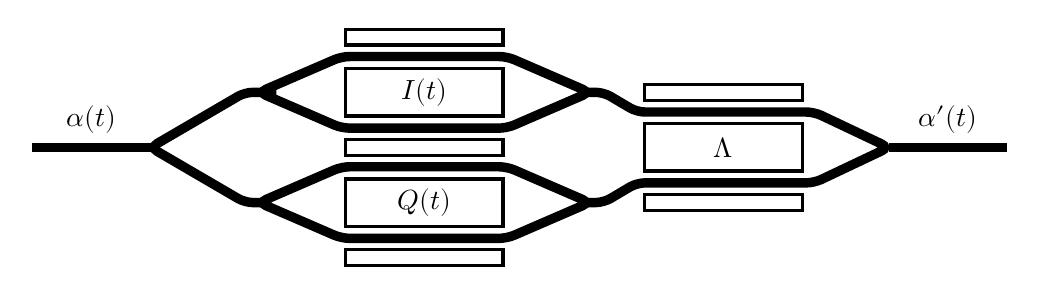
\begin{tikzpicture}[
		electrode/.style={very thick},
		waveguide/.style={line width=1.2mm, rounded corners=1mm},
	]
		\draw[electrode] (0,2.8) rectangle ++(2,0.2);
		\draw[electrode] (0,1.9) rectangle ++(2,0.6) node[pos=0.5] {$I(t)$};
		\draw[electrode] (0,1.4) rectangle ++(2,0.2);
		\draw[electrode] (0,0.5) rectangle ++(2,0.6) node[pos=0.5] {$Q(t)$};
		\draw[electrode] (0,0) rectangle ++(2,0.2);

		\draw[waveguide] (1,0.8) node[draw, regular polygon, regular polygon sides=6, minimum width=1.05cm, xscale=4] (mzm1) {};
		\draw[waveguide] (1,2.2) node[draw, regular polygon, regular polygon sides=6, minimum width=1.05cm, xscale=4] (mzm2) {};
		
		\draw[electrode] (3.8,1.2) rectangle ++(2,0.6) node[pos=0.5] {$\Lambda$};
		\draw[electrode] (3.8,0.7) rectangle ++(2,0.2);
		\draw[electrode] (3.8,2.1) rectangle ++(2,0.2);

		\path (6.9,1.5) coordinate (out);
		\path (mzm1.east)
			++(-0.3,0) coordinate (a1) 
			++(0.2,0) coordinate (b1)
			(3.7,1.05) coordinate (c1) 
			++(2.25,0) coordinate (d1);
		\path (mzm2.east-|a1) coordinate (a2)
				(a2-|b1) coordinate (b2)
				(3.7,1.95) coordinate (c2)
				(c2-|d1) coordinate (d2);

		\draw[waveguide] (a1) -- (b1) -- (c1) -- (d1) -- (out) -- (d2) -- (c2) -- (b2) -- (a2);

		\draw[waveguide] (mzm1.west) ++(0.3,0) -- ++(-0.2,0) -- ++(-1.2,0.7) coordinate (in) -- ++(1.2,0.7) -- ++(0.2,0) -- ++(0.2,0) (mzm2.west);
		
		\draw[waveguide] (in) -- ++(-1.5,0) node[midway, above] {$\alpha(t)$};
		\draw[waveguide] (out) -- ++(1.5,0) node[midway, above] {$\alpha^\prime(t)$};
	\end{tikzpicture}
\end{document}